\chapter{The Formulation of Classical Mechanics}
\section{Lagrangian formulation}
\[S=\int_{t_1}^{t_2}L(q_i,\dot{q_i},t)dt, \ \ \ \ \delta q_i(t_1) = \delta q_i(t_2) = 0.\]
\[\delta S=0 \rightarrow \frac{d}{dt}(\frac{\partial L}{\partial \dot{q_i}}) - \frac{\partial L}{\partial q_i}=0.\]

\begin{enumerate}
\item If we transform the coordinates $q$ to the $Q$ as $q = q(Q,t)$, the new Lagrangian will be
\[\bar{L}(Q,\dot{Q},t) \equiv L(q(Q,t),\dot{q}(Q,\dot{Q},t),t).\]
We can verify that
\[\frac{d}{dt}\frac{\partial \bar{L}}{\partial \dot{Q}} - \frac{\partial \bar{L}}{\partial Q} = 0.\]
\item If $L_1 = L + \frac{d}{dt} f(q,t)$, then $L$ and $L_1$ is equivalent and will generate the same dynamical equation.
\end{enumerate}

\begin{example}
\begin{enumerate}
\item The form of Lagrangian for an isolated system of particles in inertial frame:
\[L=\sum_a \frac{1}{2}m_a v_a^2 -U(\bm{r}_1,\bm{r}_2,\cdots).\]
The equation of motion is
\[m_i \ddot{\bm{r}}_i = -\nabla_{\bm{r}_i} U.\]
To get the form of Lagrangian for a system of interacting particles, we must assume:
\begin{itemize}
\item Space and time are homogeneous and isotropic in inertial frame;
\item Galileo's relativity principle and Galilean transformation;
\item Spontaneous interaction between particles;
\end{itemize}
\item Consider a reference frame $K$. Suppose the $K$ is moving with the velocity $\bm{V}(t)$ and  rotating with angular velocity $\bm{\Omega}$  relative to the inertial reference frame. We use the coordinates of the mass point in $K$ as general coordinates, i.e. $\bm{r} = (x_k,y_k,z_k)$. Then the Lagrangian of the mass point will be
\[L = \frac{1}{2}m\bm{v}^2 + m\bm{v}\cdot(\bm{\Omega}\times\bm{r})+\frac{m}{2}(\bm{\Omega}\times\bm{r})^2 - m\dot{\bm{V}}\cdot\bm{r}-U.\]
The equation of motion will be
\[m\frac{d\bm{v}}{dt} = -\frac{\partial U}{\partial \bm{r}} - m\dot{\bm{V}} + m(\bm{r} \times \dot{\bm{\Omega}}) + 2m(\bm{v} \times \bm{\Omega}) + m[\bm{\Omega}\times(\bm{r} \times \bm{\Omega})].\]
\end{enumerate}
\end{example}

\section{Symmetry and Conservation Laws(1)}
\begin{newthem}[Nother's theorem]
For $q_i \to q_i+\delta q_i$ and $L \to L+\delta L$, if $\delta L= \frac{d f(q,\dot{q},t)}{dt}$,then we get
\[\frac{d}{dt}(\sum_i p^i \delta q_i-f)=0 \ \ \ (p^i  \equiv  \frac{\partial L}{\partial \dot{q_i}}).\]
\end{newthem}
\begin{example}
For an isolated system of particles in inertial frame,\\ 
$\delta L = 0$ when $\delta \bm{r}_i \rightarrow \bm{r}_i + \delta \bm{a}$, so
\[\frac{d}{dt} (\sum_i \bm{p}_i) = 0.\]
$\delta L = 0$ when $\delta \bm{r}_i \rightarrow \bm{r}_i + \bm{r}_i \times \delta \bm{\theta}$, so
\[\frac{d}{dt} (\sum_i \bm{r}_i \times \bm{p}_i) = 0.\]
\end{example}

\paragraph{Homogeneity of time}
If $\frac{\partial L}{\partial t}=0$, then we get
\[\frac{dE}{dt}=0 \ \ \ (E=\sum_i \dot{q_i}p^i-L).\]

\section{Hamilton formulation}
\[p^i = \frac{\partial L}{\partial \dot{q_i}};\]
\[H(q,p,t)=\sum_i p^i \dot{q_i}-L;\]
\[\dot{p^i}=-\frac{\partial H}{\partial q_i}, \quad \dot{q_i}=\frac{\partial H}{\partial p^i}.\]
\begin{example}
 For an isolated system of particles in inertial frame, 
\[\bm{p}_i = m_i \bm{v}_i;\]
\[H(q,p,t)=\sum_i \frac{p_i^2}{2m} + U(\bm{r}_1,\bm{r}_2,\cdots);\]
\[\dot{\bm{p}}_i =-\nabla_{\bm{r}_i} U, \quad \dot{\bm{r}}_i = \frac{\bm{p}_i}{m_i}.\]
\end{example}
 
\subsection{Poisson Brackets}
First, we assume the bracket operation has the following properties:
\[ \left[f,g\right]=-\left[g,f\right] ;\]
\[\left[\alpha_1 f_1+\alpha_2 f_2,\beta_1 g_1+\beta_2 g_2\right]=\alpha_1 \beta_1\left[f_1,g_1\right]
+\alpha_1 \beta_2\left[f_1,g_2\right]+\alpha_2 \beta_1\left[f_2,g_1\right]+\alpha_2 \beta_2\left[f_2,g_2\right];\]
\[\left[f_1 f_2,g_1 g_2\right]=f_1\left[f_2,g_1\right]g_2+g_1 f_1\left[f_2,g_2\right]+g_1\left[f_1,g_2\right]f_2 +\left[f_1,g_1\right]g_2 f_2 ;\]
\[\left[f,\left[g,h\right]\right]+\left[g,\left[h,f\right]\right]+\left[h,\left[f,g\right]\right]=0.\]
Here, $f,g,h$ are functions of $p^i,q_i,t$.
If we assume that
\[\left [q_i,p^k\right ]=\delta^{k}_{i},\]
we can derive that 
\[ \left[f,g\right]=\sum_k(\frac{\partial f}{\partial q_k} \frac{\partial g}{\partial p^k} - \frac{\partial f}{\partial p^k} \frac{\partial g}{\partial q_k}  ).\]
Thus the Hamilton equation can be written as
\[\dot{p^i}=\left[ p^i,H \right] , \quad \dot{q_i}=\left[ q_i,H \right].\]
And we can also get
\[\frac{df}{dt} = [f,H] + \frac{\partial f}{\partial t}, \quad \frac{d}{dt} [f,g] = [\frac{df}{dt},g] + [f,\frac{dg}{dt}].\]
\begin{example}
For an isolated system of particles in inertial frame, we have
\[[r_{ia},p_{jb}] = \delta_{ab} \delta_{ij}.\]
Define $l_a \equiv \epsilon_{abc} r_{a} p_{b}$, we have
\[[l_a,r_b] = \epsilon_{abc}r_c ,\quad [l_a,p_b] = \epsilon_{abc}p_c ,\quad [l_a,l_b] = \epsilon_{abc}l_c.\]
\end{example}

\subsection{Canonical transformations}
In Hamiltonian mechanics, a canonical transformation is a change of canonical coordinates that preserves the form of Hamilton's equations (that is, the new Hamilton's equations resulting from the transformed Hamiltonian may be simply obtained by substituting the new coordinates for the old coordinates), although it might not preserve the Hamiltonian itself. 
\[Q_i = Q_i(p,q,t) ,\quad P_i=P_i(p,q,t);\]
\[\dot{Q}_i = \frac{\partial H'}{\partial P_i} ,\quad \dot{P}_i = -\frac{\partial H'}{\partial Q_i}.\]

\begin{newprop}[Canonical condition]
If $(q_i,p^i,H) \to (Q_i,P^i,H')$ is a canonical transformation, then there exists a generating function $F(q_i,Q_i,t)$ satisfying that
\[\sum_i p^i\dot{q}_i-H(p^i,q_i) = \sum_i P^i\dot{Q_i} - H'(Q_i,P^i) + \frac{dF}{dt}.\]
\end{newprop}

Applying Legendre transformation, we can get four kinds of generating function. 
\begin{enumerate}
\item \[\frac{dF}{dt} = \sum_i p^i \dot{q}_i - \sum_i P^i \dot{Q}^i + (H'-H).\]
Assume $\Phi(q_i,Q_i,t) = F$, so
\[p^i = \frac{\partial \Phi}{\partial q_i} ,\quad P^i = -\frac{\partial \Phi}{\partial Q_i} ,\quad H' = H + \frac{\partial \Phi}{\partial t}.\]

\item \[\frac{d}{dt}(F+\sum_i P^i Q_i) = \sum_i p^i \dot{q}_i + \sum_i Q_i \dot{P}^i + (H'-H).\]
Assume $\Phi(q_i,P^i,t) = F + \sum_i P^i Q_i$, so
\[p^i = \frac{\partial \Phi}{\partial q_i} ,\quad Q_i = \frac{\partial \Phi}{\partial P^i} ,\quad H' = H + \frac{\partial \Phi}{\partial t}.\]

\item \[\frac{d}{dt}(F-\sum_i p^i q_i) = -\sum_i q_i \dot{p}^i - \sum_i P^i \dot{Q}_i + (H'-H).\]
Assume $\Phi(p^i,Q_i,t) = F - \sum_i p^i q_i$, so
\[q_i = -\frac{\partial \Phi}{\partial p^i} ,\quad P^i = -\frac{\partial \Phi}{\partial Q_i} ,\quad H' = H + \frac{\partial \Phi}{\partial t}.\]

\item \[\frac{d}{dt}(F+\sum_i P^i Q_i-\sum_i p^i q_i) = -\sum_i q_i \dot{p}^i + \sum_i Q_i \dot{P}^i + (H'-H).\]
Assume $\Phi(p^i,P^i,t) = F+\sum_i P^i Q_i-\sum_i p^i q_i$, so
\[q_i = -\frac{\partial \Phi}{\partial p^i} ,\quad Q_i = \frac{\partial \Phi}{\partial P^i} ,\quad H' = H + \frac{\partial \Phi}{\partial t}.\]
\end{enumerate}

\begin{newthem}[The invariance of Poisson Bracket]
Suppose that $(q,p,H) \to (Q,P,H')$ is a canonical transformation and $f(q,p,t) = F(Q,P,t)$, $g(q,p,t) = G(Q,P,t)$, then
\[[f,g]_{q,p} = [F,G]_{Q,P}.\]
\end{newthem}
As a result, the condition for canonical transformation can also be stated as
\[[Q_i,Q_j]_{q,p} = 0, \quad [P^i,P^j]_{p,q} = 0, \quad [Q_i,P^j]_{q,p} = \delta_i^j.\]

\subsection{Evolution as canonical transformations}
Let $q_t$,$p_t$ be the values of the canonical variables at time $t$, and $q_{t+\tau}$,$p_{t+\tau}$ their values at another time $t+\tau$. The latter are some functions of the former:
\[q_{t+\tau} = q(q_t,p_t,t,\tau) ,\quad p_{t+\tau} = p(q_t,p_t,t,\tau).\]
If these formulae are regarded as a transformation from the variables $q_t$,$p_t$ to $q_{t+\tau}$, $p_{t+\tau}$, then this transformation is canonical. This is evident from the expression
\[dS = p_t dq_t + p_{t+\tau} dq_{t+\tau} -(H_{t+\tau}-H_t)dt \]
for the differential of the action $S(q_t,q_{t+\tau},t,\tau)$, taken along the true path, passing through the points $q$, and $q_{t+\tau}$ at times $t$ and $t+\tau$ for a given $\tau$. $-S$ is the generating function of the transformation. 
Thus we have the following commutation relation
\[[q_{i\,t+\tau},q_{j\,t+\tau}]_{q_t,p_t} = 0, \quad [p^i_{t+\tau},p^j_{t+\tau}]_{q_t,p_t} = 0, \quad [q_{i\,t+\tau},p^j_{t+\tau}]_{q_t,p_t} = \delta_i^j.\]

\subsection{Liouville's theorem}
\begin{newlemma}
Let $D$ be the Jacobian of the canonical transformation 
\[\frac{\partial(Q_1,\cdots,Q_s,P^1,\cdots,P^s)}{\partial(q_1,\cdots,q_s,p^1,\cdots,p^s)}.\]
Then we have
\[D=1.\]
\end{newlemma}

\begin{newthem}[Liouville's theorem]
The phase-space distribution function is constant along the trajectories of the system
\end{newthem}

\begin{newproof}
The phase volume is invariant under canonical transformation.The change in $p$ and $q$ during the motion can be regarded as a canonical transformation. Suppose that each point in the region of phase space moves in the course of time in accordance with the equations of motion of the mechanical system. The region as a whole therefore moves also, but its volume remains unchanged.
\end{newproof}

\section{Symmetry and Conservation Laws(2)}
Suppose $g$ is a function of $p$ and $q$. If the transformation of $q$ and $p$ can be described as
\[q \rightarrow q + \epsilon [q,g];\]
\[p \rightarrow p + \epsilon [p,g].\]
We can prove that 
\[H \rightarrow H + \epsilon[H,g].\]
Thus if $H$ is invariant under the transformation, then $[H,g] = 0$, that means $dg/dt = 0$, i.e. $g$ is a conserved quantity of the motion.

\section{Hamilton-Jacobi equation}
We define
\[S(q,t)=\left. \int_{q_0,t_0}^{q,t} L dt\right|_{\mathrm{extremum}}.\]
We can prove that
\[p = \frac{\partial S}{\partial q}, \ \ \ \ H = -\frac{\partial S}{\partial t}.\]
Therefore, we have
\[-\frac{\partial S}{\partial t} = H (q,\frac{\partial S}{\partial q}).\]
This is called Hamiltonian-Jacobi equation.\\ \\
Suppose the complete integral of the Hamilton-Jacobi equation is
\[S=f(t,q_1,\cdots,q_s;\alpha^1,\cdots,\alpha^s)+A,\]
where $\alpha^1,\cdots,\alpha^s$ and $A$ are arbitrary constants. 
We effect a canonical transformation from the variables $q$, $p$ to new variables, taking the function $f(t,q,\alpha)$ as the generating function, and the quantities $\alpha^1,\cdots,\alpha^s$ as the new momenta.
Let the new co-ordinates be $\beta_1,\cdots,\beta_2$, and we have
\[p^i = \frac{\partial f}{\partial q_i} ,\quad \beta_s = \frac{\partial f}{\partial \alpha_s} ,\quad H' = H + \frac{\partial f}{\partial t} =0.\]
Therefore,
\[\alpha^s = \mbox{ constant }, \beta_s = \mbox{ constant }.\]
By means of the $s$ equations $\beta_s = \partial f / \partial \alpha^s$, the $s$ coordinates $q$ can be expressed in terms of the time and the $2s$ constants. This gives the general integral of the equations of motion.

\section{Symmetry and Conservation Laws(3)}
If $S$ is invariant under transformation $q_i \rightarrow q_i + \delta q_i$, then 
\[\delta S = (\sum_i p^i \delta q_i) |_{q_0,t_0}^{q,t} = 0.\]
Therefore, we have
\[\frac{d}{dt} (p^i \delta q_i) = 0.\]
Further more, if
\[\delta S = (\sum_i p^i \delta q_i) |_{q_0,t_0}^{q,t} =  f(q_i,\dot{q}_i,t)|_{q_0,t_0}^{q,t}, \]
we will have conserved quantity
\[\frac{d}{dt} (p^i \delta q_i -f) = 0.\]

\chapter{Two Body Problem}
\section{Reduced mass and central field}
The Lagrangian for a two-body system is
\[L = \frac{1}{2} m_1 \dot{\bm{r}}_1^2 + \frac{1}{2} m_2 \dot{\bm{r}}_2^2 + U(|\bm{r}_1 - \bm{r}_2|).\]
Let $\bm{r} \equiv \bm{r}_1 -\bm{r}_2 $ be the relative position vector and let the origin be at the centre of mass, i.e. $m_1\bm{r}_1 + m_2\bm{r}_2 = 0$. These two equations give
\[\bm{r}_1 = \frac{m_2}{m_1+m_2}\bm{r} ,\quad \bm{r}_2 = \frac{m_1}{m_1+m_2}\bm{r}.\]
Then, we have
\[L = \frac{1}{2} m \dot{\bm{r}}^2 - U(r),\]
where
\[m \equiv \frac{m_1m_2}{m_1+m_2}.\]
is called reduced mass.The Lagrangian is formally identical with the Lagrangian of a particle of mass $m$ moving in an external field $U(r)$ which is symmetrical about a fixed origin. 
\\ \\
$L$ is isotropic, so angular momentum is conserved, i.e. $\bm{M} = \bm{r} \times \bm{p} = \mbox{ const }$. Since $\bm{r}$ is always perpendicular to $\bm{M}$, the path of the particle lies in one plane. Using polar coordinates, we have
\[L = \frac{1}{2}m(\dot{r}^2 + r^2 \dot{\phi}^2)-U(r).\]
It is easy to note that
\[M = mr^2\dot{\phi} = \mbox{ const }, \quad E = \frac{1}{2}m \dot{r}^2 + \frac{M^2}{2mr^2} + U(r) = \mbox{ const }.\]
Therefore,
\[\frac{dr}{dt} = \sqrt{\frac{2(E-U(r))}{m} - \frac{M^2}{m^2r^2}};\]
\[\frac{d\phi}{dr} = \frac{M}{r^2 \sqrt{2m(E-U(r))-M^2/r^2}}.\]
The radial part of the motion can be regarded as taking place in one dimension in a field where the effective potential energy is
\[U_{\mathrm{eff}} = U(r) + \frac{M^2}{2mr^2}.\]
The values of $r$ for which
\[U(r) + \frac{M^2}{2mr^2} = E \]
determine the limits of the motion as regards distance from the centre. When equation above is satisfied, the radial velocity $\dot{r}$ is zero. This does not mean that the particle comes to rest as in true one-dimensional motion, since the angular velocity is not zero. The value $\dot{r} = 0$ indicates a turning point of the path, where $r(t)$ begins to decrease instead of increasing, or vice versa.
If the range in which $r$ may vary is limited only by the condition $r \ge r_{\mathrm{min}}$, the motion is infinite: the particle comes from, and returns to, infinity.
If the range of r has two limits $r_{\mathrm{min}}$ and $r_{\mathrm{max}}$, the motion is finite and the path lies entirely within the annulus bounded by the circles $r = r_{\mathrm{min}}$ and $r = r_{\mathrm{max}}$. This does not mean that the path must be a closed curve. During the time in which $r$ varies from $r_{\mathrm{min}}$ to $r_{\mathrm{max}}$ and back, the radius vector turns through an angle
\[\Delta \phi = 2 \int_{r_{\mathrm{min}}}^{r_{\mathrm{max}}} \frac{M}{r^2 \sqrt{2m(E-U(r))-M^2/r^2}} dr.\]
The condition for the path to be closed is that this angle should be a rational fraction of $2\pi$. There are only two types of central field in which all finite motions take place in closed paths. They are those in which the potential energy of the particle varies as ${1}/{r}$ or as $r^2$.
The presence of the centrifugal energy when $M \neq 0$, which becomes infinite as ${1}/{r^2}$ when $r \to 0$, generally renders it impossible for the particle to reach the centre of the field, even if the field is an attractive one. 
A fall of the particle to the centre is possible only if the potential energy tends sufficiently rapidly to $-\infty$ as $r \to 0$. From the inequality
\[\frac{1}{2} m\dot{r}^2 = E - U(r) - \frac{M^2}{2mr^2} > 0,\]
it follows that $r$ can take values tending to zero only if
\[[r^2 U(r)]_{r\to 0} < -\frac{M^2}{2m}.\]

\section{Kepler Problem}
An important class of central fields is formed by those in which the potential energy is inversely proportional to $r$. They include the fields of $N$ Newtonian gravitational attraction and of Coulomb electrostatic interaction; the latter may be either attractive or repulsive.
\\ \\
Let us first consider an attractive field, where
\[U = -\frac{\alpha}{r} \]
with $\alpha$ a positive constant. The effective potential energy is
\[U_{\mathrm{eff}} = -\frac{\alpha}{r} + \frac{M^2}{2mr^2}.\]
As $r \to 0$, $U_{\mathrm{eff}}$ tends to $+\infty$, and as $r \to \infty$ it tends to zero from negative values; for $r = {M^2}/{m\alpha}$ it has a minimum value
\[U_{\mathrm{eff},\mathrm{min}} = -\frac{m\alpha^2}{2M^2}.\]
The motion is finite for $-{m\alpha^2}/{2M^2} \leq E < 0$ and infinite for $E \ge 0$.
The shape of path is
\[\frac{p}{r} = 1 + e \cos \phi, \]
where
\[p = \frac{M^2}{m\alpha}, \quad e = \sqrt{1 + \frac{2EM^2}{m \alpha^2}}.\]
This is the equation of a conic section with one focus at the origin; $2p$ is called the latus rectum of the orbit and $e$ the eccentricity. Our choice of the origin is such that the point where $\phi = 0$ is the point nearest to the origin (called the perihelion).
If $E < 0$,  the orbit is an ellipse and the motion is finite.
\begin{figure}[!h]
	\centering
	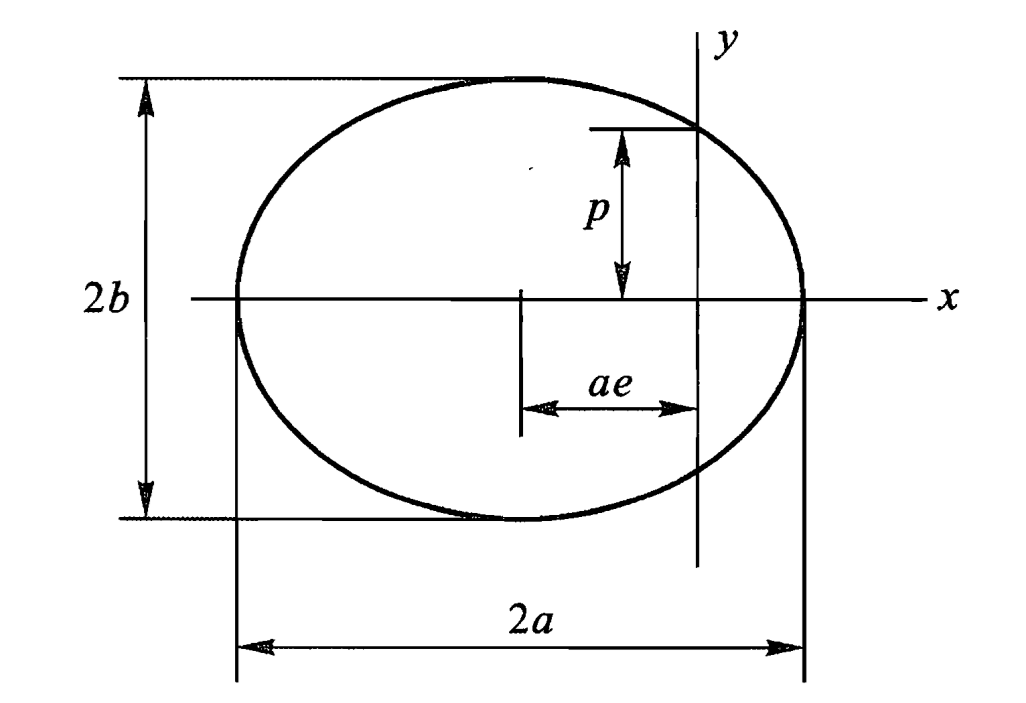
\includegraphics[height=3.5cm ,width=5cm]{CM/kepler1.png}
	\caption{Attractive Kepler orbit with $e < 1$}
\end{figure}
\\
The major and minor semi-axes of the ellipse are
\[a = \frac{p}{1-e^2} = \frac{\alpha}{2|E|} ;\quad b = \frac{p}{\sqrt{1-e^2}} = \frac{M}{\sqrt{2m|E|}}.\]
The least and greatest distances from the centre of the field (the focus of the ellipse) are
\[r_{\mathrm{min}} = \frac{p}{1+e} = a(1-e) ;\quad r_{\mathrm{max}} = \frac{p}{1-e} = a(1+e).\]
The period of revolution in an elliptical orbit is
\[T = \frac{\pi a b}{\frac{1}{2}r^2 \dot{\phi}} = 2\pi a^{3/2}\sqrt{\frac{m}{\alpha}} = \pi \alpha \sqrt{\frac{m}{2|E|^3}}.\]
\\
If $E > 0$, the path is a hyperbola with the origin as internal focus. 
\begin{figure}[!h]
	\centering
	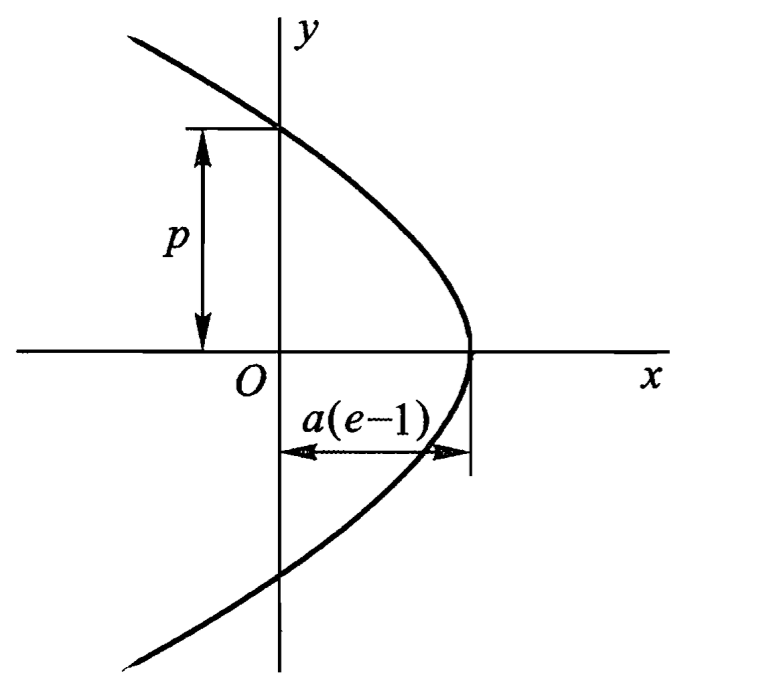
\includegraphics[height=3.5cm ,width=3.8cm]{CM/kepler2.png}
	\caption{Attractive Kepler orbit with $e > 1$}
\end{figure}
The distance of the perihelion from the focus is
\[r_{\mathrm{min}} = \frac{p}{1+e} = a(1-e),\]
where $a = {p}/{(1-e^2)^2} = {\alpha}/{2E}$ is the semiaxis of the hyperbola.
\\ \\
If $E = 0$, the eccentricity $e = 1$, and the particle moves in a parabola with perihelion distance $r_{\mathrm{min}} = {p}/{2}$. This case occurs if the particle starts from rest at infinity.
\\ \\
Let us now consider motion in a repulsive field, where
\[U= \frac{\alpha}{r} \quad (\alpha > 0).\]
Here the effective potential energy is
\[U_{\mathrm{eff}} = \frac{\alpha}{r} + \frac{M^2}{2mr^2} \]
and decreases monotonically from $+\infty$ to zero as $r$ varies from zero to infinity.
The energy of the particle must be positive, and the motion is always infinite. The calculations are exactly similar to those for the attractive field.
The path is a hyperbola:
\[\frac{p}{r} = -1 + e\cos\phi.\]
\begin{figure}[!h]
	\centering
	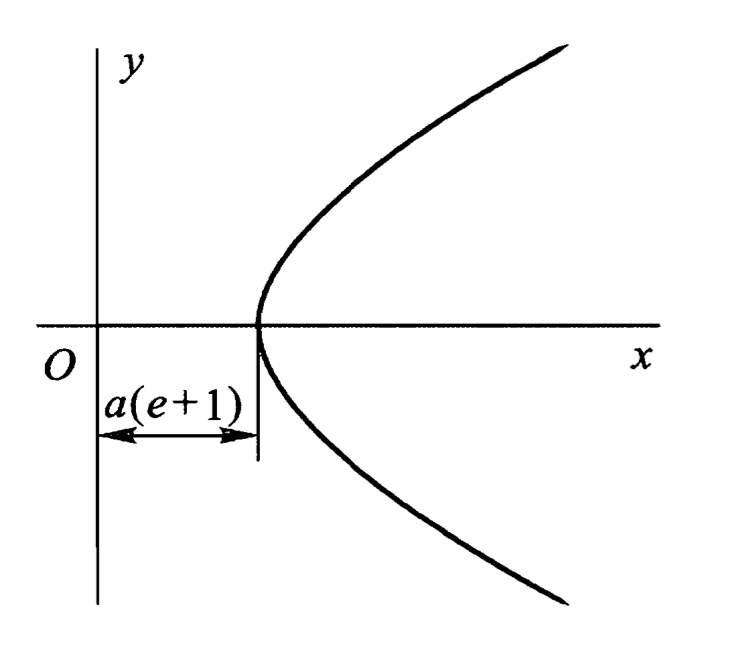
\includegraphics[height=3.3cm ,width=3.7cm]{CM/kepler3.png}
	\caption{Repulsive Kepler orbit}
\end{figure}
\\
The perihelion distance is
\[r_{\mathrm{min}} = \frac{p}{-1+e} = a(1+e).\]
\\
There is an integral of the motion which exists only in fields $U = {\alpha}/{r}$. 
It is easy to verify by direct calculation that the quantity
\[\bm{v}\times\bm{M} + \frac{\alpha \bm{r}}{r} \]
is constant. The direction of the conserved vector is along the major axis from the focus to the perihelion, and its magnitude is $\alpha e$. This is most simply seen by considering its value at perihelion.

\section{Disintegration and collisions of particles}
Let us consider a spontaneous disintegration of a particle into two constituent parts. 
This process is most simply described in a frame of reference in which the particle is at rest before the disintegration.
The law of conservation of momentum shows that the sum of the momenta of the two particles formed in the disintegration is then zero; that is, the particles move apart with equal and
opposite momenta. The magnitude $p_0$ of either momentum is given by the law of conservation of energy:
\[E_i = E_{1i} + \frac{p_0^2}{2m_1} + E_{2i} + \frac{p_0^2}{2m_2}, \]
where $m_1$ and $m_2$ are the masses of the particles, $E_{1i}$ and $E_{2i}$, their internal energies, and $E_{i}$ the internal energy of the original particle. If $\epsilon$ is the disintegration energy, i.e. the difference
\[\epsilon = E_i - E_{1i} - E_{2i} \]
which must obviously be positive, then
\[\epsilon = \frac{p_0^2}{2m}, \]
where $m$ is the reduced mass of the two particles.
\\ \\
Let us now change to a frame of reference in which the primary particle moves with velocity $\bm{V}$ before the break-up.
This frame is usually called the laboratory system, or L system, in contradistinction to the centre-of-mass
system, or C system, in which the total momentum is zero. 
Let us consider one of the resulting particles, and let $\bm{v}$ and $\bm{v}_0$ be its velocities in the L and
the C system-respectively. 
\begin{figure}[!h]
	\centering
	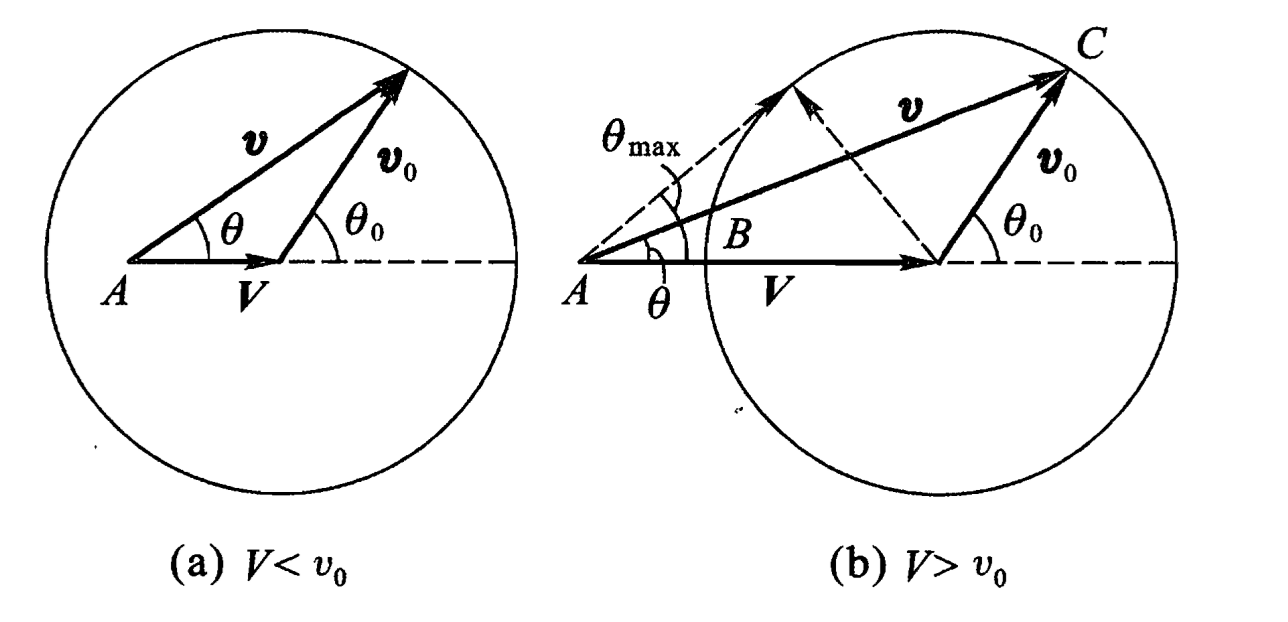
\includegraphics[height=4.5cm ,width=9.5cm]{CM/disintegration.png}
	\caption{Disintegration in L and C frame}
\end{figure}
\noindent
The relation between the angles $\theta$ and $\theta_0$ in the L and C systems is evidently,
\[\tan\theta = \frac{v_0\sin\theta_0}{V+v_0\cos\theta_0}.\]
In physical applications we are usually concerned with the disintegration of not one but many similar particles, and this raises the problem of the distribution of the resulting particles in direction, energy, etc. 
We shall assume that the primary particles are randomly oriented in space, i.e. isotropically on average.
\\ \\
In the C system, every resulting particle has the same energy, and their directions of motion are isotropically distributed. The fraction of particles entering a solid angle element $do$ is $\frac{do}{4\pi}$. 
Thus the distribution with respect to the angle $\theta_0$ is
\[\frac{1}{2}\sin\theta_0 d\theta_0.\]
The corresponding distributions in the L system are obtained by an appropriate transformation. For example, let us work out the kinetic energy distribution in the L system.
Since
\[v^2 = V^2 + v_0^2 + 2Vv_0\cos\theta_0,\] 
we have $d(v^2) = d\cos\theta_0$. Thus the kinetic energy can distributed uniformly over between $T_{\mathrm{min}} = \frac{1}{2}(v_0-V)^2$ and $T_{\mathrm{max}}= \frac{1}{2}m(v_0+V)^2$.
\\ \\
A collision between two particles is said to be elastic if it involves no change in their internal state. The collision is most simply described in the C system.The velocities of the particles before the collision are related to their velocities $\bm{v}_1$ and
$\bm{v}_2$ in the L system by $\bm{v}_{10} = m_2\bm{v}/(m_1+m_2)$, $\bm{v}_{20} = -m_1\bm{v}/(m_1+m_2)$,
where $\bm{v} = \bm{v}_1-\bm{v}_2$.
Because of the law of conservation of momentum, the momenta of the two particles remain equal and opposite after the collision, and are also unchanged in magnitude, by the law of conservation of energy. 
Thus, in the C system the collision simply rotates the velocities, which remain opposite in direction and unchanged in magnitude. The velocities of the two particles after the collision are
\[\bm{v}'_{10} = \frac{m_2v\bm{n}_0}{m_1+m_2}, \quad \bm{v}'_{20} = -\frac{m_1v\bm{n}_0}{m_1+m_2}.\]
The velocities in the L system after the collision are therefore
\[\bm{v}'_{1} = \frac{m_2v\bm{n}_0}{m_1+m_2} + \frac{m_1\bm{v_1}+m_2\bm{v_2}}{m_1+m_2}, \quad \bm{v}'_{2} = -\frac{m_1v\bm{n}_0}{m_1+m_2} + \frac{m_1\bm{v_1}+m_2\bm{v_2}}{m_1+m_2}.\]
Multiplying equations by $m_1$ and $m_2$ respectively, we obtain
\[\bm{p}'_{1} = mv\bm{n}_0 + \frac{m_1(\bm{p}_1 + \bm{p}_2)}{m_1+m_2}, \quad \bm{p}'_{2} = -mv\bm{n}_0 + \frac{m_2(\bm{p}_1 + \bm{p}_2)}{m_1+m_2}.\]
\begin{figure}[!h]
	\centering
	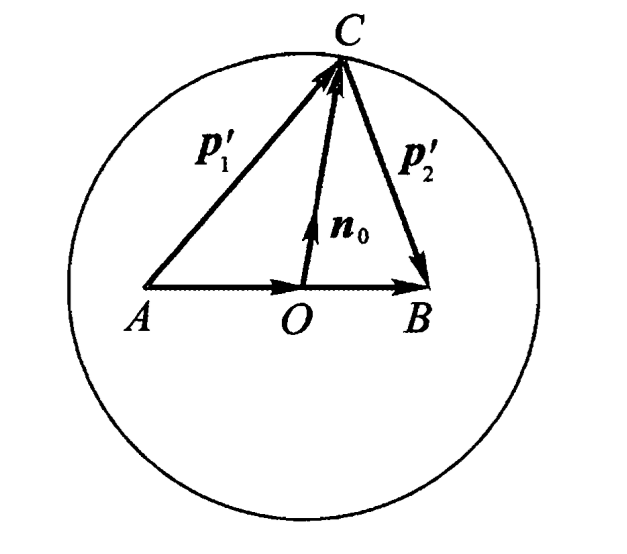
\includegraphics[height=3cm ,width=3.3cm]{CM/collision1.png}
	\caption{Collision in L and C frame}
\end{figure}
\noindent
Let us consider in more detail the case where one of the particles ($m_2$, say) is at rest before the collision. In that case the distance $OB = {m_2p_1}/{(m_1+m_2)} = mv$ is equal to the radius. The vector $\vec{AB}$ is equal to the momentum $\bm{p}_1$ of the particle $m_1$ before the collision.
\begin{figure}[!h]
	\centering
	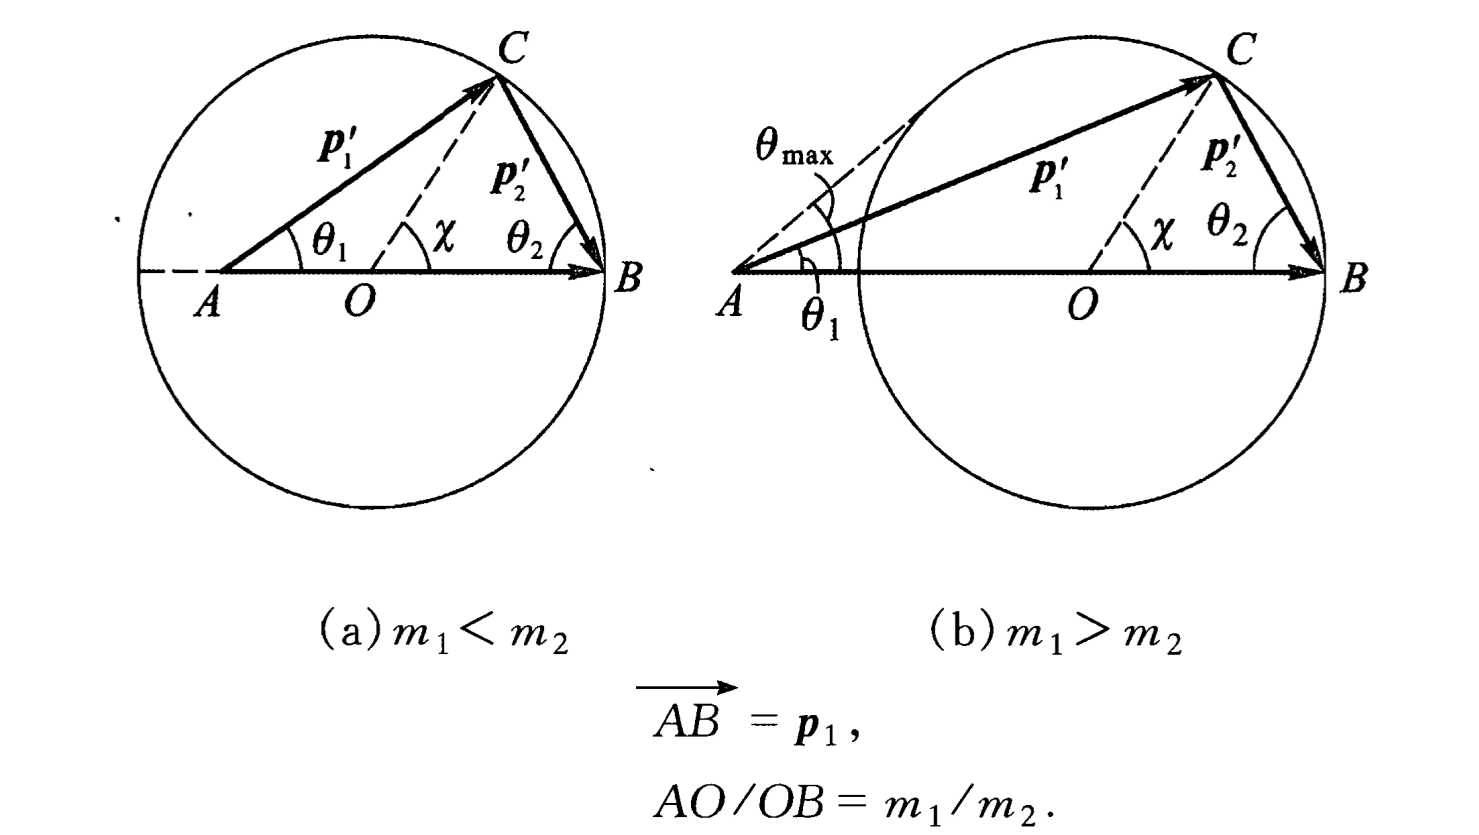
\includegraphics[height=4.2cm ,width=7.5cm]{CM/collision2.png}
	\caption{Collision with 2 at rest}
\end{figure}
\noindent
$\theta_1$ and $\theta_2$ can be expressed in terms of $\chi$ by
\[\tan\theta_1 = \frac{m_2\sin\chi}{m_1 + m_2 \cos\chi} \quad \theta_2 = \frac{1}{2}(\pi - \chi).\]
The magnitudes of the velocities of the two particles after the collision in terms of $\chi$ are
\[v'_1 = \frac{\sqrt{m_1^2 + m_2^2 + 2m_1m_2\cos\chi}}{m_1+m_2}v \quad v'_2 = \frac{2m_1v}{m_1+m_2}\sin\frac{1}{2}\chi.\]
If $m_1 < m_2$, the velocity of $m_1$ after the collision can have any direction.
If $m_1 > m_2$, this particle can be deflected only through an angle not exceeding $\theta_\mathrm{max}$ from its original direction. Evidently
\[\sin\theta_{\mathrm{max}} = \frac{m_2}{m_1}.\]
The collision of two particles of equal mass, of which one is initially at rest, is especially simple. In this case both B and A lie on the circle.
\begin{figure}[!h]
	\centering
	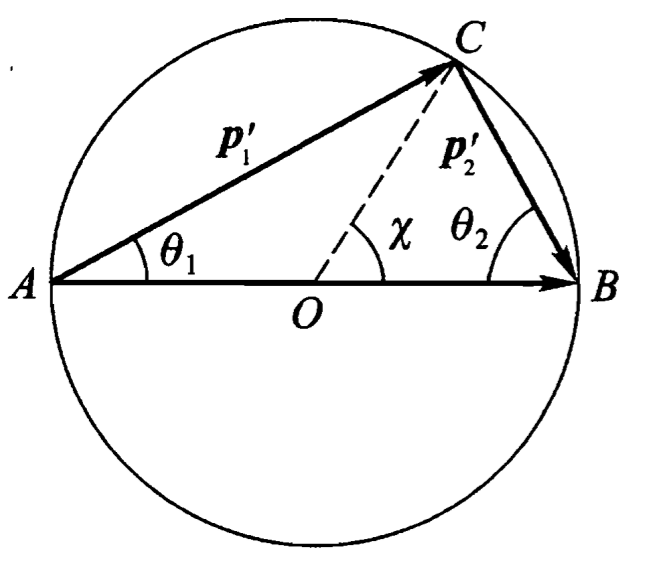
\includegraphics[height=2.9cm ,width=3.25cm]{CM/collision3.png}
	\caption{Collision of equal mass}
\end{figure}
\[\theta_1 = \frac{1}{2}\chi ,\quad \theta_2 = \frac{1}{2}(\pi-\chi);\]
\[v'_1 = v\cos\frac{1}{2}\chi ,\quad v'_2 = v\sin\frac{1}{2}\chi.\]
After the collision the particles move at right angles to each other.

\section{Scattering and cross section}
Scattering is a general physical process where some forms of radiation, such as light, sound, or moving particles, are forced to deviate from a straight trajectory by one or more paths due to localized non-uniformities in the medium through which they pass.  In classical mechanics, scattering generally refer to particle-particle collisions.
The definition of cross section  of a scattering process is
\[\sigma \equiv \frac{\mbox{Number of Events per target}}{\mbox{Time} \times \mbox{Incident Flux}}.\]
Here, the incident flux are measured in the frame of target particle. Recall that when we reduce two body problem in to one body problem, $\bm{r} = \bm{r}_1 - \bm{r}_2$ is the coordinates of projectile in the frame of target. Thus the scattering process can be represented by the reduced mass moving in the central field. 
\begin{figure}[!h]
	\centering
	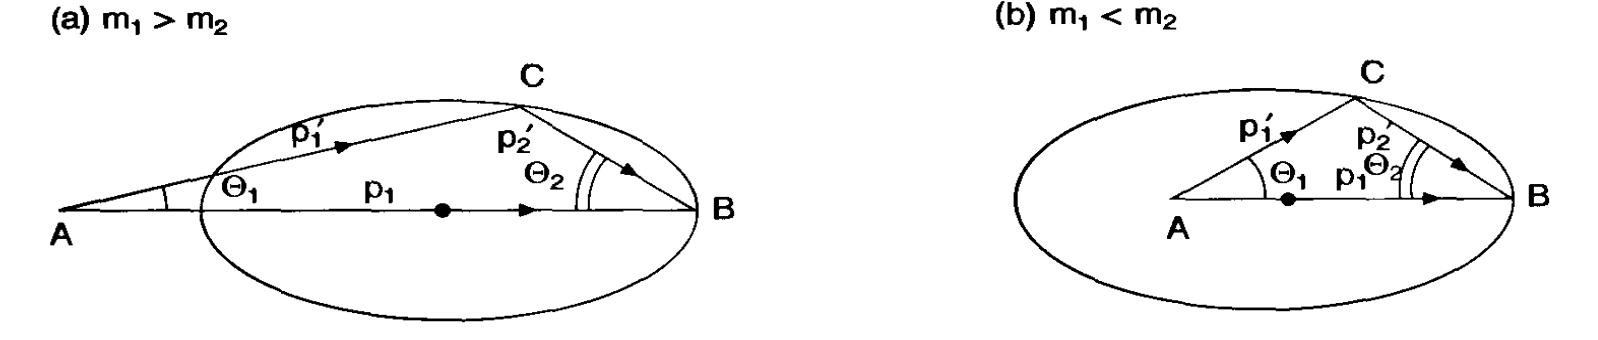
\includegraphics[height=3.9cm ,width=5.2cm]{CM/scattering.png}
	\caption{Scattering in central field}
\end{figure}
\\
And we have
\[\phi_0 = \int_{r_{\mathrm{min}}}^{\infty} \frac{Mdr}{r^2 \sqrt{2m(E-U(r))-\frac{M^2}{r^2}}} ,\quad \chi = |\pi - 2\phi_0|.\]
Since
\[E = \frac{1}{2}m v_{\infty}^2 ,\quad M = m\rho v_{\infty},\]
we can get the relation between  $\chi$ and $\rho$. Suppose the number density of the particles is $n$, then the incident flux is $nv_{\infty}$, number of events that particles are scattered into the solid angle $do = \sin\chi d\chi d\phi$ at $(\chi,\phi)$ in time $T$ is
\[d\rho \rho(\chi) d\phi nv_{\infty} T .\]
Therefore, we have
\[d\sigma = \rho(\chi) d\rho d\phi = \frac{\rho(\chi)}{\sin\chi} \left| \frac{d\rho}{d\chi} \right| do.\]
In C system, we have $\bm{r}_1 = {m_2 \bm{r}}{(m_1+m_2)} $, so the scattering angle of particle 1 is the same as $\chi$. While in L system (particle 2 is at rest before scattering), we must making corresponding transformation to get the right expression for cross section.

\subsubsection{Rutherford's formula}
One of the most important applications of the formulae derived above is to the scattering of charged particles in a Coulomb field. As $U = {\alpha}/{r}$, we have
\[\phi_0 = \arccos \frac{\alpha/mv^2_{\infty}\rho}{\sqrt{1+(\alpha/mv^2_{\infty}\rho)^2}}.\]
Recall that $\chi = (\pi-\phi_0)/2$, we can obtain that
\[\rho^2 = \frac{\alpha^2}{m^2v_{\infty}^4} \cot^2 \frac{1}{2}\chi \]
and
\[d\sigma = \left( \frac{\alpha}{2mv_{\infty}^2} \right)^2 \frac{do}{\sin^4 \frac{1}{2}\chi}.\]
This is Rutherford's formula. It may be noted that the effective cross-section is independent of the sign of $\alpha$, so that the result is equally valid for repulsive and attractive Coulomb fields.
\\ \\
Formula above gives the effective cross-section in the frame of reference in which the centre of mass of the colliding particles is at rest. The transformation to the laboratory system is effected by means of
\[\tan\theta_1 = \frac{m_2\sin\chi}{m_1 + m_2 \cos\chi} ,\quad \theta_2 = \frac{1}{2}(\pi - \chi).\]
For particles initially at rest, we have
\[d\sigma_2 = \left ( \frac{\alpha}{mv^2_{\infty}} \right )^2 \frac{do_2}{\cos^3 \theta_2}.\]
The same transformation for the incident particles leads, in general, to a very complex formula, and we shall merely note two particular cases.
\\ \\
If the mass $m_2$ of the scattering particle is large compared with the mass $m_1$ of the scattered particle, then $\chi = \theta_1$ and $m = m_1$, so that
\[d\sigma_1 = \left ( \frac{\alpha}{4E_1}\right )^2 \frac{do_1}{\sin^4 (\frac{1}{2}\theta_1)} ,\]
where $E_1 = m_1v^2_{\infty}/2$ is the energy of the incident particle.
If the masses of the two particles are equal, then by $\theta_1 = {\chi}/{2}$, we have
\[d\sigma_1 =  \left ( \frac{\alpha}{E_1}\right )^2 \frac{\cos\theta_1}{\sin^4\theta_1} do_1.\]
If the particles are entirely identical, that which was initially at rest cannot be distinguished after the collision. The total effective cross-section for all
particles is obtained by adding $do_1$ and $do_2$, so
\[d\sigma = \left ( \frac{\alpha}{E_1}\right )^2 \left ( \frac{1}{\sin^4\theta} + \frac{1}{\cos^4\theta} \right )\cos\theta do.\]
Let us return to the general formula and use it to determine the distribution of the scattered particles with respect to the energy lost in the collision. 
When the masses of the scattered and scattering particles are arbitrary, the velocity acquired by the latter is given in terms of the angle of scattering in the C system by
\[v'_2 = \frac{2m_1}{m_1+m_2} v_{\infty} \sin \frac{\chi}{2}.\]
The energy acquired by 2 and lost by 1 is therefore
\[\epsilon = \frac{2m^2}{m_2} v_{\infty}^2 \sin^2 \frac{\chi}{2} .\]
Expressing $\sin \frac{\chi}{2}$ in terms of $\epsilon$, we obtain
\[d\sigma = 2\pi \frac{\alpha^2}{m_2 v^2_{\infty}} \frac{d\epsilon}{\epsilon^2}.\]
This is the required formula: it gives the effective cross-section as a function, of the energy loss $\epsilon$, which takes values from zero to $\epsilon_{\mathrm{max}} = 2m^2 v_{\infty}^2 /m_2$.

\chapter{Small Oscillation}
\section{Small oscillation in one dimensional}
Let us consider the motion in one dimension, the potential energy of the particle is $V = V(q)$. If we choose the coordinate of equilibrium point as $q=0$, then $ \frac{\partial V}{\partial q} |_{q=0} = 0$. Expand $V(q)$ around $q=0$, we have
\[V(q) = V(0) + \frac{1}{2}  \frac{\partial^2 V}{\partial q^2} |_{q=0} \; q^2 + \cdots  \]
If the equilibrium point is stable, we have
\[\frac{\partial^2 V}{\partial q^2} |_{q=0} \equiv V''(0) > 0.\]
For small oscillation, we can neglect the higher orders of $q$ and the Lagrangian can be written as
\[L = \frac{1}{2}m\dot{q} - \frac{1}{2}V''(0)q^2.\]
The Euler-Lagrangian equation is
\[\ddot{q} + \omega_0^2 q = 0 ,\quad \omega_0^2 = \frac{V''(0)}{m}.\]
The general solution is
\[q = A\cos(\omega_0 t + \phi).\]
$A$ and $\phi$ depends on the initial condition. 
\\ \\
If there is a damped force which is proportional to the velocity of the particle, then we have
\[\ddot{q} + \frac{1}{Q}\dot{q} + \omega_0^2 q = 0.\]
If $Q > {1}/{2\omega_0}$, we have
\[q = A e^{-\frac{t}{2Q}} \cos(\omega t + \phi) ,\quad \omega = \sqrt{\omega_0^2 - \frac{1}{4Q^2}}.\]
It is called under damped oscillation.
If $Q < {1}/{2\omega_0}$, we have
\[q = Ae^{\lambda_+ t} + B Ae^{\lambda_- t},\]
where
\[\lambda_{\pm} = -\frac{1}{2Q} \pm \sqrt{\frac{1}{4Q^2} - \omega_0^2 }.\]
It is called over damped oscillation.
If $Q = {1}/{2\omega_0}$, we have
\[q = C(1+Dt)e^{-\omega_0 t}.\]
It is called critical damped oscillation.

\section{Forced oscillation}
The equation of motion for forced oscillation is
\[\ddot{q} + \frac{1}{Q}\dot{q} + \omega_0^2 q = F(t).\]
The form of solution is
\[q = q_{\mathrm{s}} + q_{\mathrm{g}} \]
and $q_{\mathrm{g}}$ is the general solution of the homogeneous equation and $q_{\mathrm{s}}$ is an arbitrary special solution of the equation. In order to get $q_{\mathrm{s}}$, we consider the following equation
\[\ddot{G} + \frac{1}{Q}\dot{G} + \omega_0^2 G = \delta(t-t') \]
and its solution is $G(t,t')$.
Then we have
\[q_{\mathrm{s}} = \int_{-\infty}^{\infty} F(t')G(t-t')dt'.\]
For under damped oscillation, we have
\[G(t,t') = \begin{cases} \frac{e^{-\frac{t-t'}{2Q}}}{\omega} \sin\omega(t-t') ,\quad t>t'\\ 0 ,\quad t<t'\end{cases} \]
and so
\[q_{\mathrm{s}} = \int_{0}^{\infty} F(t-t') \frac{e^{-\frac{t'}{2Q}}}{\omega} \sin\omega t' dt'.\]
A special case is that
\[F(t) = F_0 \cos\Omega t ,\]
and we have
\[q(t) = \frac{F_0}{\sqrt{(\Omega^2 - \omega_0^2 + \frac{1}{2Q^2})^2 + \frac{\omega^2}{Q^2}}} \cos(\Omega t + \phi), \]
where
\[\tan \phi = \frac{\frac{\Omega}{Q}}{\omega_0^2 - \Omega^2}.\]
When
\[\Omega = \sqrt{\omega_0^2 - \frac{1}{2Q^2}},\]
we have
\[q_{\mathrm{max}} = \frac{QF_0}{\omega}.\]
It is called resonance. 

\section{Non-linear oscillation and perturbation theory}
Consider the equation of motion
\[\ddot{q} + \omega_0^2 q + \epsilon q^3 = 0.\]
Suppose $\epsilon$ is very small, then we can expand
\[q = q_0 + \epsilon q_1 + \epsilon^2 q_2 + \cdots \]
and
\[\omega = \omega_0 + \epsilon \omega_1 + \epsilon^2 \omega_2 + \cdots \]
The equation of motion can be written as
\[\ddot{q} + \omega^2 q = (\omega^2 -\omega_0^2)q - \epsilon q^3.\]
Let $\tau \equiv \omega t$ and $q' \equiv {dq}/{d\tau} = {\dot{q}}/{\omega}$, we have
\[q'' + q = (1- \frac{\omega_0^2}{\omega^2})q - \frac{\epsilon}{\omega^2} q^3 = 0.\]
We can solve the equation above power by power and get
\[q_0'' + q_0 = 0 ,\]
\[q_1'' + q_1 = -\frac{q_0^3}{\omega_0^2} + \frac{2\omega_1}{\omega_0}q_0, \]
and so on. 
When doing the perturbation, we must adjust the $\omega_i$ to avoid the resonance solution. The details will be neglect here.
\\ \\
Now let us consider the non-linear oscillation with drive force. The equation of motion is
\[\ddot{q} + \frac{1}{Q}\dot{q} + \omega_0^2 q + \epsilon q^3 = F_0 \cos \omega t.\]
It can be rewritten as
\[\ddot{q} + \omega^2 q = - \frac{1}{Q} \dot{q} + (\omega^2 - \omega_0^2)q - \epsilon q^3 + F_0\cos\omega t.\]
We treat the right hand of the equation as perturbation, so we multiply it by a parameter $\mu$ and let it be $1$ later,
\[\ddot{q} + \omega^2 q = \mu \left (- \frac{1}{Q} \dot{q} + (\omega^2 - \omega_0^2)q - \epsilon q^3 + F_0\cos\omega t \right ).\]
Concerning on the phase lagging effect, we redefine the ``time'' as 
\[\tau \equiv \omega t - \delta, \]
so 
\[q'' + q = \mu \left [ -\frac{1}{Q\omega} q' + \left ( 1- \frac{\omega_0^2}{\omega^2} \right ) q - \frac{\epsilon}{\omega^2} q^3 + \frac{F_0}{\omega^2} \cos (\tau + \delta) \right ].\]
The expansion series of $q$ and $\delta$ are
\[q = q_0 + \mu q_1 + \mu^2 q_2 + \cdots \]
\[\delta = \delta_0 + \mu \delta_1 + \mu^2 \delta_2 + \cdots \]
We can solve the equation above power by power and get
\[q''_0 + q_0 = 0,\]
\[q''_1 + q_1 =  -\frac{1}{Q\omega} q_0' + \left ( 1- \frac{\omega_0^2}{\omega^2} \right ) q_0 - \frac{\epsilon}{\omega^2} q_0^3 + \frac{F_0}{\omega^2} \cos (\tau + \delta_0), \]
and so on. 
The solution of the zeroth order perturbation is
\[q_0 = A_0 \cos\tau.\]
Substitute it into the first order equation, we have
\[q''_1 + q_1 = \left ( \frac{A_0}{Q\omega} - \frac{F_0}{\omega^2} \sin\delta_0 \right ) \sin\tau + \left [ \left ( 1 - \frac{\omega_0^2}{\omega^2}\right ) A_0 - \frac{3\epsilon A_0^3}{4\omega^2} + \frac{F_0}{\omega^2}\cos\delta_0 \right ] \cos\tau - \frac{\epsilon A_0^3}{4\omega^2} \cos 3\tau.\]
To avoid non-physical solution, we have
\[\sin\delta_0 = \frac{A_0 \omega}{F_0 Q} \]
and
\[\left ( 1 - \frac{\omega_0^2}{\omega^2}\right ) A_0 - \frac{3\epsilon A_0^3}{4\omega^2} + \frac{F_0}{\omega^2}\cos\delta_0 = 0.\]
Now, we can get
\[A_0 = \frac{F_0}{\sqrt{\left[ (\omega^2 -\omega_0^2) - \frac{3}{4}\epsilon A_0^2 \right ]^2 + \frac{\omega^2}{Q^2} }}.\]
If we define
\[x \equiv \frac{\omega}{\omega_0} ,\quad y \equiv \frac{A_0 \omega_0^2}{F_0},\]
the equation above can be written as
\[y^2 = \frac{1}{(x^2-1-ay^2)^2 + bx^2}, \]
where
\[a = \frac{3\epsilon F_0^2}{4\omega_0^6}, \quad b = \frac{1}{\omega_0^2 Q^2}.\]
We than can solve for $x$ in terms of $y$,
\[x^2 = \frac{2 + 2ay-b \pm \sqrt{(b-2-2ay)^2-4(a^2y^2+2ay+1-\frac{1}{y})}}{2}.\]
\begin{figure}[!h]
	\centering
	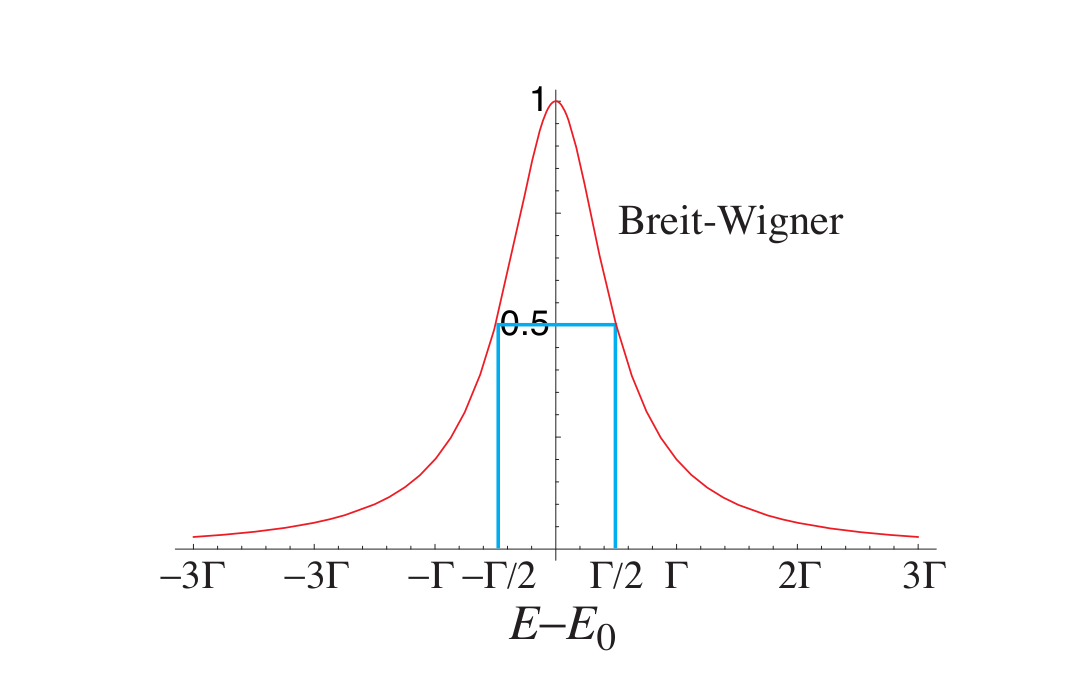
\includegraphics[height=6cm ,width=12cm]{CM/resonance.png}
	\caption{Resonance curve}
\end{figure}
\\ 
Thus the resonance curve has two branches, corresponding to the two roots of the equation above. When the frequency of the drive force increase from left, the amplitude of oscillation will become larger and larger. But when it comes to the point of inflection, the amplitude will drop to the low-right part of the curve. When the frequency of the drive force decrease from right, the amplitude of oscillation will also become larger and larger. When it comes to the point of inflection, the amplitude will jump to the hight-left part of the curve. 
This effect is called hysteresis.

\section{Oscillations of systems with more than one degree of freedom}
Let's look at a system with many degrees of freedom; we have
\[L={\frac {1}{2}}\sum _{i,j}T_{ij}{\dot {q}}_{i}{\dot {q}}_{j}-V\left(q_{1},\ldots q_{n}\right).\]
Let $q_{0,i}$ be an equilibrium position and expand about this point $q_{i}=q_{0,i}+\eta _{i}$, so $\dot{q}_{i}=\dot {\eta }_{i}$.
We can expand the potential energy to give
\[V\left(q_{1},\ldots q_{n}\right)=V\left(q_{0,1},\ldots q_{0,n}\right)+\sum _{i}\left({\frac {\partial V}{\partial q_{i}}}\right)_{q_{0,i}}\eta _{i}+{\frac {1}{2}}\sum _{i,j}\left({\frac {\partial ^{2}V}{\partial q_{i}\partial q_{j}}}\right)_{q_{0,i}}\eta _{i}\eta _{j}+\cdots \]
The first term is a constant with respect to $\eta_i$ and constant terms do not affect the motion. The second term is zero, because $q_{0,i}$ is a point of equilibrium so we are left with
\[L={\frac {1}{2}}\sum _{i,j}\left(T_{ij}{\dot {\eta }}_{i}{\dot {\eta }}_{j}-V_{ij}\eta _{i}\eta _{j}\right), \]
where
\[T_{ij}=T_{ij}\left(q_{0,1},\ldots q_{0,n}\right) ,\quad V_{ij}=\left({\frac {\partial ^{2}V}{\partial q_{i}\partial q_{j}}}\right)_{q_{0,i}},\]
yielding the equations of motion
\[\sum _{j}\left(T_{ij}{\ddot {\eta }}_{j} + V_{ij}\eta _{j}\right)=0.\]
This is a linear differential equation with constant coefficients. We can try the solution
\[\eta _{i}=Ca_{i}e^{-i\omega t}.\]
Thus we have
\[\sum _{j}\left(V_{ij}a_{j}-\omega ^{2}T_{ij}a_{j}\right)=0.\]
This is a matrix equation such that
\[{\vec {\vec {A}}}\cdot {\vec {a}}=0 \]
with
\[{\vec {a}}=\left[{\begin{matrix}a_{1}\\a_{2}\\\vdots \\a_{j}\end{matrix}}\right] \]
and
\[{\vec {\vec {A}}}=\left[{\begin{matrix}V_{11}-\omega ^{2}T_{11}&V_{12}-\omega ^{2}T_{12}&\cdots \\V_{21}-\omega ^{2}T_{21}&V_{22}-\omega ^{2}T_{22}&\cdots \\\vdots &&\end{matrix}}\right].\]
This equation only has a solution is $\det {\vec {\vec {A}}}=0$. This gives a $n$th-degree polynomial to solve for $\omega^2$. We will get $n$ solutions for $\omega^2$ that we can substitute into the matrix equation and solve for $a_j$.

\chapter{Motion of a Rigid Body}
\section{Angular velocity}
Suppose there are two coordinate frames. The frame 2 is rotating with respect to frame 1. If the coordinates of a particle in frame 2 are $r_2=(x_2,y_2,z_2)$.
Then the coordinates of the particle in frame 1 are
\[r_1 = O(t)r_2 ,\]
and we have
\[O^TO=I.\]
Note that
\[\Omega + \Omega^T= 0 ,\quad \Omega \equiv O^T\frac{dO}{dt}.\]
It is easy to derive that
\[\frac{dr_1}{dt} = \frac{dO}{dt}r_2 + O\frac{dr_2}{dt} = OO^T \frac{dO}{dt}r_2 + Ov_2  = O (\Omega r_2 + v_2) ,\quad v_2 \equiv \frac{dr_2}{dt}.\]
Suppose
\[\Omega = \left[ \begin{matrix} 0& -\omega_{2z}& \omega_{2y}\\ \omega_{2z}& 0& -\omega_{2x}\\ -\omega_{2y}& \omega_{2x}& 0\end{matrix} \right] .\]
We can get
\[v_1 \equiv \frac{dr_1}{dt}  = O(\omega_2 \times r_2 + v_2) .\]
Now, we define
\[\omega_1 \equiv O\omega_2.\]
We can verify that
\[O \Omega O^T = \left[ \begin{matrix} 0& -\omega_{1z}& \omega_{1y}\\ \omega_{1z}& 0& -\omega_{1x}\\ -\omega_{1y}& \omega_{1x}& 0\end{matrix} \right] .\]
Therefore, we have
\[v_1 = \omega_1 \times r_1 + Ov_2 ,\]
where $\omega$ is the so-called angular velocity.
\begin{note}
$\omega_1$ is independent of the base vector we choose for frame 2.
If we choose frame 1 differently, $\omega_1$ will transform like an vector.
\end{note}

\section{Dynamics of rigid body}
\subsubsection{Inertial tensor of rigid body}
Suppose there is frame attached to the rigid body, then the coordinate of all the mass point of the rigid body is constant in this frame, i.e.
\[r_1 = r_0(t) + O(t)r_2 ,\quad r_2 \mbox{ is a constant}.\]
Thus we have
\[v_1 = V + \omega_1 \times r_1 = V + O(\omega_2 \times r_2).\]
The kinetic energy of the rigid body is
\[T = \sum \frac{m}{2} (\bm{V} + \bm{\omega} \times \bm{r})^2 = \sum \frac{m}{2} V^2 + \sum m\bm{V}\cdot(\bm{\omega}\times\bm{r}) + \sum \frac{m}{2} (\bm{\omega} \times \bm{r})^2.\]
If we choose the origin of the frame 2 to be the center of mass of the rigid body, we have
\[T = \frac{\mu V^2}{2} + \frac{1}{2}\sum m [\omega^2r^2-(\bm{\omega} \cdot \bm{r})^2].\]
If we define the inertial tensor as
\[I_{ik} = \sum m (x_l^2 \delta_{ik} - x_i x_k),\]
the kinetic energy of the rigid body can be rewritten as
\[T = \frac{\mu V^2}{2} + \frac{1}{2} I_{ik}\omega_i \omega_k ,\]
and the Lagrangian of the rigid body is
\[L = \frac{\mu V^2}{2} + \frac{1}{2} I_{ik}\omega_i \omega_k -U.\]
If the body is regarded as continuous, the sum becomes an integral over the volume of the body:
\[I_{ik} = \int \rho (x_l^2 \delta_{ik} - x_i x_k) dV.\]
Like any symmetrical tensor of rank two, the inertia tensor can be reduced to diagonal form by an appropriate choice of the directions of the axes $x_1$, $x_2$ $x_3$. 
These directions are called the principal axes of inertia, and the corresponding values of the diagonal components of the tensor are called the principal moments of inertia; we shall denote them by $I_1$, $I_2$, $I_3$. 
When the axes $x_1$, $x_2$ $x_3$ are so chosen, the kinetic energy of rotation takes the very simple form
\[T_{\rm rot} = \frac{1}{2} (I_1 \omega_1^2 + I_2 \omega_2^2 + I_3 \omega_3^2).\]
\\ \\
A body whose three principal moments of inertia are all different is called an asymmetrical top. 
If two are equal ($I_1 = I_2 \neq I_3$), we have a symmetrical top. 
In this case the direction of one of the principal axes in the $x_1x_2$-plane may be chosen arbitrarily.
If all three principal moments of inertia are equal, the body is called a spherical top, and the three axes of inertia may be chosen arbitrarily as any three mutually perpendicular axes.
\\ \\
The determination of the principal axes of inertia is much simplified if the body is symmetrical, for it is clear that the position of the centre of mass and the directions of the principal axes must have the same symmetry as the body.
For example, if the body has a plane of symmetry, the centre of mass must lie in that plane, which also contains two of the principal axes of inertia, while the third is perpendicular to the plane.
If a body has an axis of symmetry of any order, the centre of mass must lie on that axis, which is also one of the principal axes of inertia, while the other two are perpendicular to it.
If the axis is of order higher than the second, the body is a symmetrical top. For any principal axis perpendicular to the axis of symmetry can be turned through an angle different from $\pi$ about the latter, i.e. the choice of the perpendicular axes is not unique, and this can happen only if the body is a symmetrical top.
\\ \\
Finally, we may note one further result concerning the calculation of the inertia tensor. 
Although this tensor has been defined with respect to a system of co-ordinates whose origin is at the centre of mass , it may sometimes be more conveniently found by first calculating a similar tensor,
\[I'_{ik} = \sum m (x_l^{'2} \delta_{ik} - x'_i x'_k), \]
defined with respect to some other origin $O'$. 
If the distance $OO'$ is represented by a vector $\bm{a}$, then $\bm{r} = \bm{r'} + \bm{a}$; since, by the definition
of $O$, $\sum m\bm{r} = 0$, we have
\[I'_{ik} = I_{ik} + \mu (a^2\delta_{ik}-a_i a_k).\]
Using this formula, we can easily figure out $I_{ik}$ if $I'_{ik}$ is known.

\subsubsection{Angular momentum}
The value of the angular momentum of systems depends on the point with respect to which it is defined. In the mechanics of a rigid body, the most appropriate point to choose for this purpose is the origin of the moving system of co-ordinates, i.e. the centre of mass of the body. Then we have
\[\bm{M} = \sum m\bm{r} \times (\bm{\omega} \times \bm{r} + \bm{V}) = \sum m \left [ r^2\bm{\omega} - (\omega \cdot \bm{r})\bm{r} \right ],\]
or, in tensor notation,
\[M_i = I_{ik}\omega_k.\]
If the axes $x_1$, $x_2$ $x_3$ are the same as the principal axes of inertia, we have
\[M_1 = I_1 \omega_1 ,\quad M_2 = I_2 \omega_2 ,\quad M_3 = I_3 \omega_3.\]

\subsubsection{Equation of motion}
Since a rigid body has, in general, six degrees of freedom, the general equations of motion must be six in number. They can be put in a form which gives the time derivatives of two vectors, the momentum and the angular momentum of the body.
The first equation is obtained by simply summing the equations $\dot{\bm{p}} = \bm{f}$ for each particle in the body. In terms of the total momentum of the body
\[\bm{P} = \sum \bm{p} = \mu\bm{V}, \]
and total force acting on it $\bm{F} = \sum \bm{f}$, we have
\[\frac{d\bm{P}}{dt} = \bm{F} .\]
Although $\bm{F}$ has been defined as the sum of all the forces $\bm{f}$ acting on the various particles, including the forces due to other particles, $\bm{F}$ actually includes only external forces: the forces of interaction between the particles composing the body must cancel out, since if there are no external forces the momentum of the body, like that of any closed system, must be conserved, i.e. we must have $\bm{F} = 0$. 
\\ \\
Let us now derive the second equation of motion, which gives the time derivative of the angular momentum $\bm{M}$.
To simplify the derivation, it is convenient to choose the fixed (inertial) frame of reference in such a way that the centre of mass is at rest in that frame at the instant considered. We have
\[\dot{\bm{M}} = \frac{d}{dt} \sum \bm{r} \times \bm{p} = \sum \bm{\dot{r}} \times \bm{p} + \sum \bm{r} \times \dot{\bm{p}}.\]
Our choice of the frame of reference (with $\bm{V} = 0$) means that the vectors $\dot{\bm{r}}$ and $\bm{p} = m\bm{v}$ are parallel, so $\dot{\bm{r}} \times \bm{p} = 0$. We have
\[\frac{d\bm{M}}{dt} = \bm{K}, \]
where
\[\bm{K} = \sum \bm{r} \times \bm{f}.\]
Since $\bm{M}$ has been defined as the angular momentum about the centre of mass, it is unchanged when we go from one inertial frame to another. We can therefore deduce that the equation of motion, though derived for a particular frame of reference, is valid in any other inertial frame, by Galileo's relativity principle.
The vector $\bm{r}\times \bm{f}$ is called the moment of the force $\bm{f}$, and so $\bm{K}$ is the total torque, i.e. the sum of the moments of all the forces acting on the body. Like the total force, $\sum \bm{r} \times \bm{f}$ need include only the external forces: by the law of conservation of angular momentum, the sum of the moments of the internal forces in a closed system must be zero.

\subsubsection{Euler's equations}
Let ${d\bm{A}}/{dt}$ be the rate of change of any vector $\bm{A}$ with respect to the fixed system of co-ordinates. We have
\[\frac{d\bm{A}}{dt} = \frac{d'\bm{A}}{dt} + \bm{\omega} \times \bm{A}, \]
where
${d'\bm{A}}/{dt}$ is the rate of change of the $\bm{A}$'s components in the body system of coordinates. Therefore, we have
\[\frac{d'\bm{M}}{dt} + \bm{\omega} \times \bm{M} = \bm{K}.\]
Suppose the principal axes of inertia are $x_1$, $x_2$ $x_3$, so we have
\begin{eqnarray}
I_1 \frac{d\omega_1}{dt} + (I_3-I_2)\omega_2\omega_3 &=& K_1 ;\nonumber \\
I_2 \frac{d\omega_2}{dt} + (I_1-I_3)\omega_1\omega_3 &=& K_2 ;\nonumber \\
I_3 \frac{d\omega_1}{dt} + (I_2-I_1)\omega_1\omega_2 &=& K_3 .\nonumber
\end{eqnarray}
These are called Euler's equations.

\section{Eulerian angle}
The motion of a rigid body can be described by means of the three co-ordinates of its centre of mass and any three angles which determine the orientation of the axes $x_1$, $x_2$ $x_3$ in the moving system of coordinates relative to the fixed system $X$, $Y$, $Z$. These angles may often be conveniently taken as what are called Eulerian angles.
\begin{figure}[!h]
	\centering
	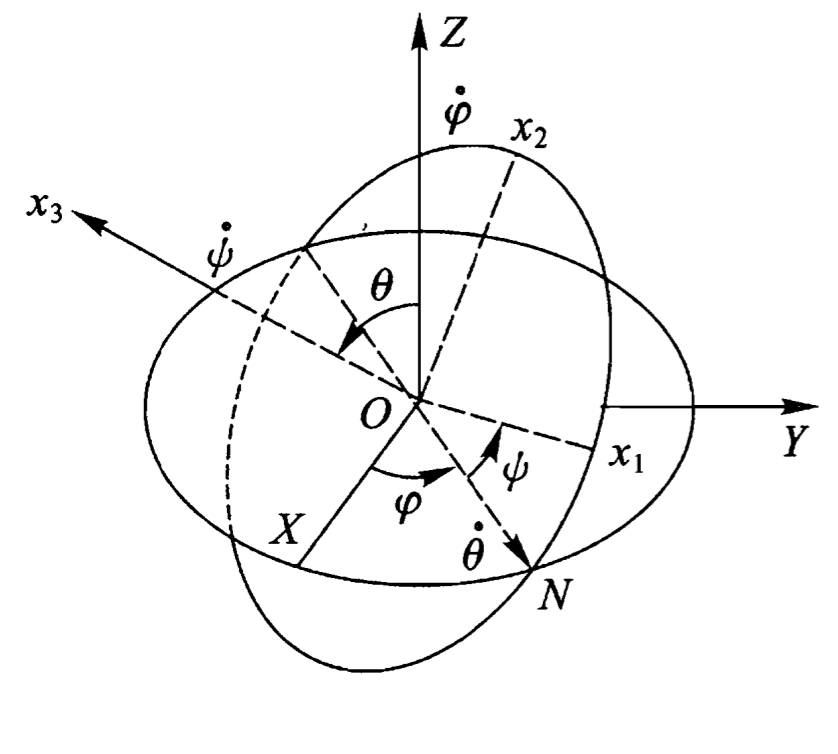
\includegraphics[height=5.7cm ,width=6.3cm]{CM/euler.png}
	\caption{Eulerian angle}
\end{figure}
The moving $x_1x_2$-plane intersects the fixed $XY$-plane in some line $ON$, called the line of nodes. 
This line is evidently perpendicular to both the $Z$-axis and the $x_3$-axis; we take its positive direction as that of the vector product $\bm{z} \times \bm{x}_3$.
We take, as the quantities defining the position of the axes $x_1$, $x_2$ $x_3$ relative to the axes $X$, $Y$, $Z$ the angle $\theta$ between the $Z$ and $x_3$ axes, the angle $\phi$ between the $X$-axis and $ON$, and the angle $\psi$  between the $x_1$ and $ON$.
\\ \\
Let us now express the components of the angular velocity  vector $\omega$ along the moving axes $x_1$, $x_2$ $x_3$ in terms of the Eulerian angles and their derivatives. 
To do this, we must find the components along those axes of the angular velocities $\dot{\theta}$, $\dot{\phi}$, $\dot{\psi}$. The angular velocity $\dot{\theta}$ is along the line of nodes $ON$. The angular velocity $\dot{\phi}$ is along the $Z$-axis. The angular velocity $\psi$ is along the $x_3$-axis. Collecting the components along each axis, we have
\begin{eqnarray}
\omega_1 &=& \dot{\phi}\sin\theta\sin\psi + \dot{\theta}\cos\psi; \nonumber \\
\omega_2 &=& \dot{\phi}\sin\theta\cos\psi - \dot{\theta}\sin\psi; \nonumber \\
\omega_3 &=& \dot{\phi} \cos\theta + \dot{\psi}. \nonumber
\end{eqnarray}
For a symmetrical top, by using the fact that the choice of directions of the principal axes $x_1$, $x_2$ is arbitrary for a symmetrical top. 
If the $x_1$ axis is taken along the line of nodes $ON$, i.e. $\psi = 0$, the components of the angular velocity are simply
\[\omega_1 = \dot{\theta} ,\quad \omega_2 = \dot{\phi}\sin\theta ,\quad \omega_3 = \dot{\phi}\cos\theta + \dot{\psi}.\]
For the free motion of a symmetrical top, we take the $Z$-axis of the fixed system of coordinates in the direction of the constant angular momentum $M$ of the top. The $x_3$-axis of the moving system is along the axis of the top; let the $x_1$-axis coincide with the line of nodes at the instant considered. 
Then the components of the vector $M$ are
\[M_1 = I_1\dot{\theta} ,\quad M_2 = I_2 \dot{\phi}\sin\theta ,\quad M_3 = I_3(\dot{\phi}\cos\theta + \dot{\psi}).\]
Since the $x_1$-axis is perpendicular to the $Z$-axis, we have
\[M_1 = 0 ,\quad M_2 = M\sin\theta ,\quad M_3 = M\cos\theta.\]
Comparison gives
\[\dot{\theta} = 0 ,\quad  \dot{\phi} = \frac{M}{I_1} ,\quad \dot{\phi}\cos\theta + \dot{\psi} = \frac{M\cos\theta}{I_3}.\]
The first of these equations gives $\theta = \mbox{ constant} $, i.e. the angle between the axis of the top and the direction of $\bm{M}$ is constant. The second equation gives
the angular velocity of precession $\dot{\phi} = {M}/{I_1}$. Finally, the third equation gives the angular velocity with which the top rotates about its own axis $\omega_3 = {M\cos\theta}/{I_3}$.